% ==============================================================================
% BỘ ĐỀ THAM KHẢO TUYỂN SINH 10 NĂM HỌC 2026-2027 SỞ GD&ĐT TP.HCM
% ĐỢT 23: CỤM 15 (ĐỀ 3 - ĐỀ SỐ 45) VÀ CỤM 16 (ĐỀ 1 - ĐỀ SỐ 46)
% Gồm 14 bài toán tự luận chuẩn cấu trúc tuyển sinh 10
% ==============================================================================

% ==============================================================================
% CỤM 15 - ĐỀ THAM KHẢO 3 (ĐỀ SỐ 45)
% ==============================================================================

\begin{bt}%[9D6H18-2]
% nguon: Đề tham khảo Tuyển sinh 10 năm học 2026-2027 Sở GD&ĐT TP.HCM - Cụm 15 Đề 3 (Đề số 45)
Cho hàm số $y = \dfrac{1}{4}x^2$ có đồ thị là parabol $(P)$.
\begin{enumerate}[a)]
	\item Vẽ đồ thị $(P)$ trên mặt phẳng toạ độ $Oxy$.
	\item Tìm toạ độ các điểm $M$ thuộc $(P)$ có tung độ bằng $4$.
\end{enumerate}
\loigiai{
\begin{enumerate}[a)]
	\item Bảng giá trị của hàm số:
	\begin{center}
		\begin{tabular}{|c|c|c|c|c|c|}
			\hline
			$x$ & $-4$ & $-2$ & $0$ & $2$ & $4$ \\ \hline
			$y = \dfrac{1}{4}x^2$ & $4$ & $1$ & $0$ & $1$ & $4$ \\ \hline
		\end{tabular}
	\end{center}
	Đồ thị $(P)$ là đường parabol có đỉnh tại gốc toạ độ $O(0;0)$, nhận trục $Oy$ làm trục đối xứng và quay bề lõm lên trên.
	\begin{center}
	\begin{tikzpicture}[>=stealth,scale=0.8]
		\draw[->] (-5,0) -- (5,0) node[below] {$x$};
		\draw[->] (0,-1) -- (0,5.5) node[left] {$y$};
		\node[below left] at (0,0) {$O$};
		\draw[dashed] (-4,0) node[below] {$-4$} -- (-4,4) -- (0,4) node[left] {$4$} -- (4,4) -- (4,0) node[below] {$4$};
		\draw[dashed] (-2,0) node[below] {$-2$} -- (-2,1) -- (0,1) node[left] {$1$} -- (2,1) -- (2,0) node[below] {$2$};
		\draw[thick,smooth,samples=100,domain=-4.4:4.4] plot(\x,{0.25*(\x)^2});
		\fill (-4,4) circle (1.5pt) (-2,1) circle (1.5pt) (0,0) circle (1.5pt) (2,1) circle (1.5pt) (4,4) circle (1.5pt);
		\node[right] at (3,2.5) {$(P)\colon y = \dfrac{1}{4}x^2$};
	\end{tikzpicture}
	\end{center}
	\item Vì điểm $M$ có tung độ bằng $4$ nên ta có phương trình:
	$$\dfrac{1}{4}x^2 = 4 \iff x^2 = 16 \iff x = 4 \text{ hoặc } x = -4.$$
	Vậy toạ độ các điểm cần tìm là $(4; 4)$ và $(-4; 4)$.
\end{enumerate}
}
\end{bt}

\begin{bt}%[9D6H20-2]
% nguon: Đề tham khảo Tuyển sinh 10 năm học 2026-2027 Sở GD&ĐT TP.HCM - Cụm 15 Đề 3 (Đề số 45)
Cho phương trình $-3x^2 + x + 1 = 0$.
\begin{enumerate}[a)]
	\item Chứng minh phương trình luôn có hai nghiệm phân biệt $x_1, x_2$.
	\item Không giải phương trình, hãy tính giá trị của biểu thức $A = x_1^2 + \dfrac{2}{x_1} + x_2^2 + \dfrac{2}{x_2}$.
\end{enumerate}
\loigiai{
\begin{enumerate}[a)]
	\item Phương trình $-3x^2 + x + 1 = 0$ có các hệ số $a = -3$, $b = 1$, $c = 1$.
	Ta có:
	$$\Delta = b^2 - 4ac = 1^2 - 4 \cdot (-3) \cdot 1 = 1 + 12 = 13 > 0.$$
	(hoặc do $a \cdot c = (-3) \cdot 1 = -3 < 0$ nên phương trình có hai nghiệm trái dấu).
	Vì $\Delta > 0$ nên phương trình luôn có hai nghiệm phân biệt $x_1, x_2$.
	\item Áp dụng định lý Viète, ta có:
	$$\begin{cases} x_1 + x_2 = -\dfrac{b}{a} = -\dfrac{1}{-3} = \dfrac{1}{3} \\ x_1 x_2 = \dfrac{c}{a} = \dfrac{1}{-3} = -\dfrac{1}{3}. \end{cases}$$
	Ta có:
	$$x_1^2 + x_2^2 = (x_1 + x_2)^2 - 2x_1 x_2 = \left(\dfrac{1}{3}\right)^2 - 2 \cdot \left(-\dfrac{1}{3}\right) = \dfrac{1}{9} + \dfrac{2}{3} = \dfrac{7}{9}.$$
	Biến đổi biểu thức $A$:
	$$A = (x_1^2 + x_2^2) + \left(\dfrac{2}{x_1} + \dfrac{2}{x_2}\right) = (x_1^2 + x_2^2) + \dfrac{2(x_1 + x_2)}{x_1 x_2}.$$
	Thay các giá trị tương ứng vào, ta được:
	$$A = \dfrac{7}{9} + \dfrac{2 \cdot \dfrac{1}{3}}{-\dfrac{1}{3}} = \dfrac{7}{9} + (-2) = \dfrac{7}{9} - \dfrac{18}{9} = -\dfrac{11}{9}.$$
	Vậy $A = -\dfrac{11}{9}$.
\end{enumerate}
}
\end{bt}

\begin{bt}%[9D8H26-3]
% nguon: Đề tham khảo Tuyển sinh 10 năm học 2026-2027 Sở GD&ĐT TP.HCM - Cụm 15 Đề 3 (Đề số 45)
Bạn An thực hiện một trò chơi với một hộp có $6$ quả bóng được đánh số từ $1$ đến $6$. Bạn ấy lấy ngẫu nhiên một quả bóng, ghi lại số rồi bỏ lại vào hộp và lặp lại quá trình này $40$ lần. Kết quả thu được ghi nhận số lần xuất hiện của các số như sau: số $1$ xuất hiện $5$ lần, số $2$ xuất hiện $8$ lần, số $3$ xuất hiện $7$ lần, số $4$ xuất hiện $4$ lần, số $5$ xuất hiện $6$ lần, số $6$ xuất hiện $10$ lần.
\begin{enumerate}[a)]
	\item Tính giá trị trung bình cộng của các số ghi trên quả bóng đã rút ra trong trò chơi.
	\item Tính xác suất thực nghiệm của biến cố $A$: ``Số ghi trên bóng là số chẵn''.
	\item Tính xác suất thực nghiệm của biến cố $B$: ``Số ghi trên bóng là số nguyên tố nhỏ hơn $5$''.
\end{enumerate}
\loigiai{
Tổng số lần thực hiện phép thử là:
$$n = 5 + 8 + 7 + 4 + 6 + 10 = 40\text{ (lần)}.$$
\begin{enumerate}[a)]
	\item Tổng các giá trị của các số ghi trên quả bóng rút ra là:
	$$T = 1 \cdot 5 + 2 \cdot 8 + 3 \cdot 7 + 4 \cdot 4 + 5 \cdot 6 + 6 \cdot 10 = 5 + 16 + 21 + 16 + 30 + 60 = 148.$$
	Giá trị trung bình cộng là:
	$$\bar{X} = \dfrac{148}{40} = 3{,}7.$$
	\item Các số chẵn xuất hiện trên quả bóng là $2, 4, 6$.
	Số lần xuất hiện số chẵn là:
	$$n(A) = 8 + 4 + 10 = 22\text{ (lần)}.$$
	Xác suất thực nghiệm của biến cố $A$ là:
	$$P(A) = \dfrac{n(A)}{n} = \dfrac{22}{40} = \dfrac{11}{20}.$$
	\item Các số nguyên tố nhỏ hơn $5$ trên quả bóng là $2$ và $3$.
	Số lần xuất hiện số nguyên tố nhỏ hơn $5$ là:
	$$n(B) = 8 + 7 = 15\text{ (lần)}.$$
	Xác suất thực nghiệm của biến cố $B$ là:
	$$P(B) = \dfrac{n(B)}{n} = \dfrac{15}{40} = \dfrac{3}{8}.$$
\end{enumerate}
}
\end{bt}

\begin{bt}%[9D6V21-3]
% nguon: Đề tham khảo Tuyển sinh 10 năm học 2026-2027 Sở GD&ĐT TP.HCM - Cụm 15 Đề 3 (Đề số 45)
Cô Liên có một mảnh đất hình chữ nhật kích thước $20\text{ m} \times 25\text{ m}$. Cô Liên dự định xây nhà trên một phần đất hình chữ nhật có các cạnh cách mép đất lần lượt là $x$ (m) và $x + 1$ (m), phần đất còn lại dùng để làm sân vườn.
\begin{enumerate}[a)]
	\item Viết biểu thức theo $x$ biểu diễn diện tích phần đất dùng để xây nhà và thu gọn biểu thức đó.
	\item Tìm $x$, biết diện tích phần đất làm nhà là $140\text{ m}^2$.
\end{enumerate}
\loigiai{
\begin{enumerate}[a)]
	\item Chiều rộng của phần đất xây nhà là:
	$$20 - x\text{ (m)}.$$
	Chiều dài của phần đất xây nhà là:
	$$25 - (x + 1) = 24 - x\text{ (m)}.$$
	Điều kiện: $0 < x < 20$.
	Diện tích phần đất dùng để xây nhà là:
	$$S = (24 - x)(20 - x) = 480 - 24x - 20x + x^2 = x^2 - 44x + 480\text{ (m}^2\text{)}.$$
	\item Theo giả thiết, diện tích đất làm nhà là $140\text{ m}^2$ nên ta có phương trình:
	$$x^2 - 44x + 480 = 140 \iff x^2 - 44x + 340 = 0.$$
	Biệt thức $\Delta' = (-22)^2 - 1 \cdot 340 = 484 - 340 = 144 > 0 \implies \sqrt{\Delta'} = 12$.
	Phương trình có hai nghiệm:
	$$x_1 = 22 - 12 = 10\text{ (nhận do } 0 < x < 20\text{)}; \quad x_2 = 22 + 12 = 34\text{ (loại)}.$$
	Vậy $x = 10$ m.
\end{enumerate}
}
\end{bt}

\begin{bt}%[9H0V31-3]
% nguon: Đề tham khảo Tuyển sinh 10 năm học 2026-2027 Sở GD&ĐT TP.HCM - Cụm 15 Đề 3 (Đề số 45)
Một hộp phô mai hình trụ có đường kính đáy $12{,}2\text{ cm}$, chiều cao $2{,}4\text{ cm}$. Bên trong có $8$ miếng phô mai được xếp nằm sát nhau vừa khít trong hộp.
\begin{enumerate}[a)]
	\item Tính thể tích của một miếng phô mai (làm tròn kết quả đến chữ số thập phân thứ nhất).
	\item Người ta gói từng miếng phô mai bằng một loại giấy bạc đặc biệt (vừa khít miếng phô mai). Hãy tính diện tích phần giấy gói mỗi miếng phô mai (làm tròn kết quả đến hàng đơn vị).
\end{enumerate}
\loigiai{
\begin{enumerate}[a)]
	\item Bán kính đáy của hộp phô mai hình trụ là:
	$$R = 12{,}2 : 2 = 6{,}1\text{ (cm)}.$$
	Thể tích của toàn bộ hộp phô mai là:
	$$V = \pi R^2 h = \pi \cdot (6{,}1)^2 \cdot 2{,}4 = 89{,}304\pi\text{ (cm}^3\text{)}.$$
	Vì $8$ miếng phô mai xếp vừa khít trong hộp nên thể tích của một miếng phô mai là:
	$$V_1 = \dfrac{V}{8} = \dfrac{89{,}304\pi}{8} = 11{,}163\pi \approx 35{,}1\text{ (cm}^3\text{)}.$$
	\item Mỗi miếng phô mai có dạng hình quạt trụ (góc ở tâm $45^\circ$). Diện tích toàn phần bề mặt của một miếng phô mai gồm:
	\begin{itemize}
		\item Diện tích hai mặt đáy hình quạt tròn (mỗi mặt chiếm $\dfrac{1}{8}$ diện tích đáy):
		$$S_1 = 2 \cdot \dfrac{1}{8}\pi R^2 = \dfrac{1}{4}\pi \cdot (6{,}1)^2 = 9{,}3025\pi\text{ (cm}^2\text{)}.$$
		\item Diện tích mặt cong ngoài hình trụ (chiếm $\dfrac{1}{8}$ diện tích xung quanh):
		$$S_2 = \dfrac{1}{8} \cdot 2\pi R h = \dfrac{1}{4}\pi \cdot 6{,}1 \cdot 2{,}4 = 3{,}66\pi\text{ (cm}^2\text{)}.$$
		\item Diện tích hai mặt phẳng bên (hai hình chữ nhật kích thước $R \times h$):
		$$S_3 = 2 \cdot R \cdot h = 2 \cdot 6{,}1 \cdot 2{,}4 = 29{,}28\text{ (cm}^2\text{)}.$$
	\end{itemize}
	Tổng diện tích giấy gói mỗi miếng phô mai là:
	$$S = S_1 + S_2 + S_3 = (9{,}3025\pi + 3{,}66\pi) + 29{,}28 = 12{,}9625\pi + 29{,}28 \approx 70\text{ (cm}^2\text{)}.$$
	Vậy diện tích giấy gói mỗi miếng phô mai khoảng $70\text{ cm}^2$.
\end{enumerate}
}
\end{bt}

\begin{bt}%[9D1H3-4]
% nguon: Đề tham khảo Tuyển sinh 10 năm học 2026-2027 Sở GD&ĐT TP.HCM - Cụm 15 Đề 3 (Đề số 45)
Trong phòng thực hành, hai máy in 3D (gọi là Máy $A$ và Máy $B$) được giao nhiệm vụ in hai mô hình kiến trúc giống hệt nhau. Ở chế độ bình thường, công suất in của Máy $A$ gấp đôi Máy $B$. Tuy nhiên, nếu Máy $A$ bị nóng và chuyển sang chế độ làm mát thì công suất chỉ còn bằng $\dfrac{1}{4}$ công suất bình thường của chính nó. Cả hai máy bắt đầu in cùng một lúc. Máy $B$ hoạt động ổn định từ đầu đến cuối. Máy $A$ chạy bình thường được $2$ giờ thì bị quá nhiệt và chuyển sang chế độ làm mát cho đến khi in xong. Kết quả là cả hai máy hoàn thành mô hình cùng một lúc. Hỏi tổng thời gian để in xong mô hình là bao nhiêu giờ?
\loigiai{
Gọi $x$ (mô hình/giờ) là công suất in của Máy $B$ và $y$ (giờ) là tổng thời gian in xong mô hình ($x > 0, y > 2$).
Công suất in bình thường của Máy $A$ là $2x$ (mô hình/giờ).
Công suất in ở chế độ làm mát của Máy $A$ là:
$$\dfrac{1}{4} \cdot 2x = \dfrac{1}{2}x\text{ (mô hình/giờ)}.$$
Vì Máy $B$ in xong $1$ mô hình trong $y$ giờ nên ta có phương trình:
$$xy = 1. \quad (1)$$
Máy $A$ in ở chế độ bình thường trong $2$ giờ và ở chế độ làm mát trong $y - 2$ giờ để hoàn thành $1$ mô hình:
$$2x \cdot 2 + \dfrac{1}{2}x(y - 2) = 1 \iff 4x + \dfrac{1}{2}xy - x = 1 \iff 3x + \dfrac{1}{2}xy = 1. \quad (2)$$
Thay $xy = 1$ từ $(1)$ vào $(2)$, ta được:
$$3x + \dfrac{1}{2} \cdot 1 = 1 \iff 3x = \dfrac{1}{2} \iff x = \dfrac{1}{6}.$$
Thay $x = \dfrac{1}{6}$ vào $(1)$, ta được:
$$y = \dfrac{1}{x} = 6\text{ (giờ, thoả mãn condition)}.$$
Vậy tổng thời gian để in xong mô hình là $6$ giờ.
}
\end{bt}

\begin{bt}%[9H9C29-3]
% nguon: Đề tham khảo Tuyển sinh 10 năm học 2026-2027 Sở GD&ĐT TP.HCM - Cụm 15 Đề 3 (Đề số 45)
Cho đường tròn $(O; R)$ có bán kính $R = 2{,}5\text{ cm}$, đường kính $AB$ và dây cung $AC = 4\text{ cm}$ không đi qua tâm. Hai tiếp tuyến tại $A$ và $C$ của $(O)$ cắt nhau tại $D$. Gọi $E$ là giao điểm của $OD$ và $AC$. Kẻ $CF \perp AB$ tại $F$.
\begin{enumerate}[a)]
	\item Chứng minh bốn điểm $O, A, C, D$ cùng thuộc một đường tròn và $BC \perp AC$.
	\item Chứng minh $\widehat{AOD} = \widehat{ABC}$ và $CF \cdot AB = CA \cdot CB$.
	\item Gọi $G$ là trung điểm của $CF$, $H$ là giao điểm của hai tia $AG$ và $DC$. Chứng minh $HB$ là tiếp tuyến của đường tròn $(O)$ và tính chu vi của tứ giác $ABHD$.
\end{enumerate}
\loigiai{
\begin{center}
\begin{tikzpicture}[>=stealth,scale=1.1]
	\def\R{2.5}
	\coordinate (O) at (0,0);
	\draw[thick] (O) circle (\R);
	\coordinate (A) at (-\R,0);
	\coordinate (B) at (\R,0);
	\draw (A) -- (B);
	% AC = 4, AB = 5 -> cos(BAC) = 4/5 = 0.8 -> góc khoảng 36.87 độ
	\coordinate (C) at ({\R*cos(180-2*36.87)},{\R*sin(180-2*36.87)});
	\draw (A) -- (C) -- (B);
	% Tiếp tuyến tại A và C cắt nhau tại D
	\coordinate (D) at (-\R,3.33);
	\draw (A) -- (D) -- (C);
	\draw (O) -- (D);
	\coordinate (E) at (intersection of O--D and A--C);
	% CF vuông góc AB tại F
	\coordinate (F) at ($(A)!(C)!(B)$);
	\draw (C) -- (F);
	\coordinate (G) at ($(C)!0.5!(F)$);
	% H là giao điểm AG và DC
	\coordinate (H) at (intersection of A--G and D--C);
	\draw (A) -- (H);
	\draw (D) -- (H);
	\draw (B) -- (H);
	% Ký hiệu
	\fill (O) circle (1.5pt) node[below] {$O$}
		  (A) circle (1.5pt) node[below left] {$A$}
		  (B) circle (1.5pt) node[below right] {$B$}
		  (C) circle (1.5pt) node[above] {$C$}
		  (D) circle (1.5pt) node[above left] {$D$}
		  (E) circle (1.5pt) node[above] {$E$}
		  (F) circle (1.5pt) node[below] {$F$}
		  (G) circle (1.5pt) node[left] {$G$}
		  (H) circle (1.5pt) node[above right] {$H$};
\end{tikzpicture}
\end{center}
\begin{enumerate}[a)]
	\item Vì $DA, DC$ là các tiếp tuyến của $(O)$ nên $DA \perp OA$ và $DC \perp OC$, suy ra:
	$$\widehat{OAD} = 90^\circ \text{ và } \widehat{OCD} = 90^\circ.$$
	Tứ giác $OACD$ có $\widehat{OAD} + \widehat{OCD} = 90^\circ + 90^\circ = 180^\circ$, do đó bốn điểm $O, A, C, D$ cùng thuộc đường tròn đường kính $OD$.
	Tam giác $ABC$ nội tiếp đường tròn $(O)$ có cạnh $AB$ là đường kính nên $\widehat{ACB} = 90^\circ$, suy ra $BC \perp AC$.
	\item Theo tính chất hai tiếp tuyến cắt nhau, tia $OD$ là phân giác của $\widehat{AOC}$:
	$$\widehat{AOD} = \dfrac{1}{2}\widehat{AOC}.$$
	Mặt khác, trong đường tròn $(O)$, góc nội tiếp $\widehat{ABC}$ bằng nửa góc ở tâm cùng chắn cung $AC$:
	$$\widehat{ABC} = \dfrac{1}{2}\widehat{AOC}.$$
	Do đó $\widehat{AOD} = \widehat{ABC}$.
	Tam giác $ABC$ vuông tại $C$ có đường cao $CF$, xét diện tích tam giác $ABC$:
	$$S_{\triangle ABC} = \dfrac{1}{2} CA \cdot CB = \dfrac{1}{2} CF \cdot AB \implies CF \cdot AB = CA \cdot CB.$$
	\item Ta có $DA \perp AB$ và $CF \perp AB$, suy ra $DA \parallel CF$.
	Gọi $K$ là giao điểm của tiếp tuyến tại $B$ của $(O)$ với đường thẳng $DC$, ta có $KB \perp AB \implies KB \parallel CF \parallel DA$.
	Áp dụng định lý Thales trong hình thang $ABKD$ có $G$ là trung điểm $CF$, ta chứng minh được ba điểm $A, G, K$ thẳng hàng.
	Mà $H$ là giao điểm của tia $AG$ với $DC$, nên điểm $H$ trùng với điểm $K$.
	Do đó $HB$ là tiếp tuyến của $(O)$ tại $B$, suy ra $\widehat{OBH} = 90^\circ$ và $HC = HB$.
	Tính chu vi tứ giác $ABHD$:
	Đường kính $AB = 2R = 2 \cdot 2{,}5 = 5\text{ cm}$.
	Tam giác $ABC$ vuông tại $C$ có $AB = 5\text{ cm}, AC = 4\text{ cm} \implies BC = \sqrt{5^2 - 4^2} = 3\text{ cm}$.
	Đường cao $CF = \dfrac{CA \cdot CB}{AB} = \dfrac{4 \cdot 3}{5} = 2{,}4\text{ cm} \implies CG = \dfrac{CF}{2} = 1{,}2\text{ cm}$.
	Vì $OD$ là đường trung trực của $AC$ nên $E$ là trung điểm của $AC \implies AE = 2\text{ cm}$.
	Trong tam giác vuông $OAE$ tại $E$:
	$$OE = \sqrt{OA^2 - AE^2} = \sqrt{2{,}5^2 - 2^2} = 1{,}5\text{ cm}.$$
	Áp dụng hệ thức lượng trong tam giác vuông $OAD$ tại $A$:
	$$OA^2 = OE \cdot OD \implies OD = \dfrac{OA^2}{OE} = \dfrac{2{,}5^2}{1{,}5} = \dfrac{25}{6}\text{ cm}.$$
	$$AD = \sqrt{OD^2 - OA^2} = \sqrt{\left(\dfrac{25}{6}\right)^2 - \left(\dfrac{15}{6}\right)^2} = \dfrac{20}{6} = \dfrac{10}{3}\text{ cm} \implies CD = AD = \dfrac{10}{3}\text{ cm}.$$
	Vì $CG \parallel AD$ nên $\triangle HCG \sim \triangle HDA$ (g-g):
	$$\dfrac{HC}{HD} = \dfrac{CG}{AD} \iff \dfrac{HC}{HC + CD} = \dfrac{1{,}2}{\dfrac{10}{3}} = 0{,}36 \implies HC = 0{,}36\left(HC + \dfrac{10}{3}\right) \implies HC = \dfrac{15}{8}\text{ cm}.$$
	Suy ra $HB = HC = \dfrac{15}{8}\text{ cm}$ và $HD = HC + CD = \dfrac{15}{8} + \dfrac{10}{3} = \dfrac{125}{24}\text{ cm}$.
	Chu vi tứ giác $ABHD$ là:
	$$P = AB + BH + HD + DA = 5 + \dfrac{15}{8} + \dfrac{125}{24} + \dfrac{10}{3} = \dfrac{120 + 45 + 125 + 80}{24} = \dfrac{370}{24} = \dfrac{185}{12}\text{ (cm)}.$$
	Vậy chu vi tứ giác $ABHD$ là $\dfrac{185}{12}\text{ cm}$.
\end{enumerate}
}
\end{bt}

% ==============================================================================
% CỤM 16 - ĐỀ THAM KHẢO 1 (ĐỀ SỐ 46)
% ==============================================================================

\begin{bt}%[9D6H18-2]
% nguon: Đề tham khảo Tuyển sinh 10 năm học 2026-2027 Sở GD&ĐT TP.HCM - Cụm 16 Đề 1 (Đề số 46)
Cho hàm số $y = 2x^2$ có đồ thị là parabol $(P)$.
\begin{enumerate}[a)]
	\item Vẽ đồ thị $(P)$ trên mặt phẳng toạ độ $Oxy$.
	\item Tìm toạ độ các điểm $M$ thuộc đồ thị $(P)$ có hoành độ bằng hai lần tung độ.
\end{enumerate}
\loigiai{
\begin{enumerate}[a)]
	\item Bảng giá trị của hàm số:
	\begin{center}
		\begin{tabular}{|c|c|c|c|c|c|}
			\hline
			$x$ & $-2$ & $-1$ & $0$ & $1$ & $2$ \\ \hline
			$y = 2x^2$ & $8$ & $2$ & $0$ & $2$ & $8$ \\ \hline
		\end{tabular}
	\end{center}
	Đồ thị $(P)$ là đường parabol có đỉnh tại gốc toạ độ $O(0;0)$, nhận trục $Oy$ làm trục đối xứng và quay bề lõm lên trên.
	\begin{center}
	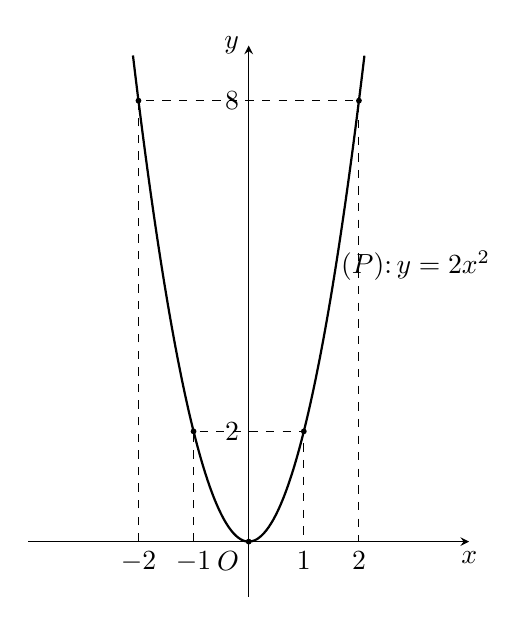
\begin{tikzpicture}[>=stealth,scale=0.7]
		\draw[->] (-4,0) -- (4,0) node[below] {$x$};
		\draw[->] (0,-1) -- (0,9) node[left] {$y$};
		\node[below left] at (0,0) {$O$};
		\draw[dashed] (-2,0) node[below] {$-2$} -- (-2,8) -- (0,8) node[left] {$8$} -- (2,8) -- (2,0) node[below] {$2$};
		\draw[dashed] (-1,0) node[below] {$-1$} -- (-1,2) -- (0,2) node[left] {$2$} -- (1,2) -- (1,0) node[below] {$1$};
		\draw[thick,smooth,samples=100,domain=-2.1:2.1] plot(\x,{2*(\x)^2});
		\fill (-2,8) circle (1.5pt) (-1,2) circle (1.5pt) (0,0) circle (1.5pt) (1,2) circle (1.5pt) (2,8) circle (1.5pt);
		\node[right] at (1.5,5) {$(P)\colon y = 2x^2$};
	\end{tikzpicture}
	\end{center}
	\item Điểm $M$ thuộc $(P)$ có hoành độ bằng hai lần tung độ nên $x = 2y \implies y = \dfrac{x}{2}$.
	Phương trình hoành độ giao điểm:
	$$\dfrac{x}{2} = 2x^2 \iff 2x^2 - \dfrac{x}{2} = 0 \iff x\left(2x - \dfrac{1}{2}\right) = 0 \iff x = 0 \text{ hoặc } x = \dfrac{1}{4}.$$
	\begin{itemize}
		\item Với $x = 0 \implies y = 0$.
		\item Với $x = \dfrac{1}{4} \implies y = \dfrac{1}{4} : 2 = \dfrac{1}{8}$.
	\end{itemize}
	Vậy toạ độ các điểm cần tìm là $(0; 0)$ và $\left(\dfrac{1}{4}; \dfrac{1}{8}\right)$.
\end{enumerate}
}
\end{bt}

\begin{bt}%[9D6H20-2]
% nguon: Đề tham khảo Tuyển sinh 10 năm học 2026-2027 Sở GD&ĐT TP.HCM - Cụm 16 Đề 1 (Đề số 46)
Cho phương trình $x^2 + x - 3 = 0$.
\begin{enumerate}[a)]
	\item Chứng minh phương trình luôn có hai nghiệm phân biệt $x_1, x_2$.
	\item Không giải phương trình, hãy tính giá trị của biểu thức $A = \dfrac{x_1 - 1}{x_2 + 1} + \dfrac{x_2 - 1}{x_1 + 1}$.
\end{enumerate}
\loigiai{
\begin{enumerate}[a)]
	\item Phương trình $x^2 + x - 3 = 0$ có các hệ số $a = 1$, $b = 1$, $c = -3$.
	Ta có:
	$$\Delta = b^2 - 4ac = 1^2 - 4 \cdot 1 \cdot (-3) = 1 + 12 = 13 > 0.$$
	Vì $\Delta > 0$ nên phương trình luôn có hai nghiệm phân biệt $x_1, x_2$.
	\item Theo định lý Viète, ta có:
	$$\begin{cases} x_1 + x_2 = -\dfrac{b}{a} = -1 \\ x_1 x_2 = \dfrac{c}{a} = -3. \end{cases}$$
	Ta có:
	$$x_1^2 + x_2^2 = (x_1 + x_2)^2 - 2x_1 x_2 = (-1)^2 - 2(-3) = 1 + 6 = 7.$$
	Biến đổi biểu thức $A$:
	\begin{align*}
		A &= \dfrac{(x_1 - 1)(x_1 + 1) + (x_2 - 1)(x_2 + 1)}{(x_2 + 1)(x_1 + 1)} \\
		&= \dfrac{(x_1^2 - 1) + (x_2^2 - 1)}{x_1 x_2 + (x_1 + x_2) + 1} \\
		&= \dfrac{(x_1^2 + x_2^2) - 2}{x_1 x_2 + (x_1 + x_2) + 1}.
	\end{align*}
	Thay các giá trị tương ứng vào, ta được:
	$$A = \dfrac{7 - 2}{-3 + (-1) + 1} = \dfrac{5}{-3} = -\dfrac{5}{3}.$$
	Vậy $A = -\dfrac{5}{3}$.
\end{enumerate}
}
\end{bt}

\begin{bt}%[9D8H26-3]
% nguon: Đề tham khảo Tuyển sinh 10 năm học 2026-2027 Sở GD&ĐT TP.HCM - Cụm 16 Đề 1 (Đề số 46)
Một hộp có chứa $10$ quả bóng cùng kích thước và khối lượng, được đánh số từ $1$ đến $10$. Lấy ra ngẫu nhiên đồng thời $2$ quả bóng trong hộp. Tính xác suất của mỗi biến cố sau:
\begin{enumerate}[a)]
	\item $A$: ``Tích hai số ghi trên hai quả bóng là một số lẻ''.
	\item $B$: ``Tổng hai số ghi trên hai quả bóng nhỏ hơn $8$''.
\end{enumerate}
\loigiai{
Số cách chọn ngẫu nhiên đồng thời $2$ quả bóng từ $10$ quả bóng là:
$$n(\Omega) = \mathrm{C}_{10}^2 = \dfrac{10 \cdot 9}{2} = 45.$$
\begin{enumerate}[a)]
	\item Tích của hai số là một số lẻ khi và chỉ khi cả hai số được chọn đều là số lẻ.
	Trong hộp có $5$ quả bóng mang số lẻ là $\{1; 3; 5; 7; 9\}$.
	Số cách chọn $2$ quả bóng mang số lẻ là:
	$$n(A) = \mathrm{C}_5^2 = \dfrac{5 \cdot 4}{2} = 10.$$
	Xác suất của biến cố $A$ là:
	$$P(A) = \dfrac{n(A)}{n(\Omega)} = \dfrac{10}{45} = \dfrac{2}{9}.$$
	\item Các cặp hai số khác nhau $\{a, b\}$ có tổng nhỏ hơn $8$ là:
	$$\{1, 2\}, \{1, 3\}, \{1, 4\}, \{1, 5\}, \{1, 6\}, \{2, 3\}, \{2, 4\}, \{2, 5\}, \{3, 4\}.$$
	Số kết quả thuận lợi cho biến cố $B$ là $n(B) = 9$.
	Xác suất của biến cố $B$ là:
	$$P(B) = \dfrac{n(B)}{n(\Omega)} = \dfrac{9}{45} = \dfrac{1}{5}.$$
\end{enumerate}
}
\end{bt}

\begin{bt}%[9D6V21-3]
% nguon: Đề tham khảo Tuyển sinh 10 năm học 2026-2027 Sở GD&ĐT TP.HCM - Cụm 16 Đề 1 (Đề số 46)
Một tấm tôn hình vuông có cạnh bằng $x$ (cm). Người ta muốn cắt tấm tôn đó để làm một cái nắp đậy hình tròn có đường kính đúng bằng cạnh của tấm tôn.
\begin{enumerate}[a)]
	\item Viết biểu thức tính diện tích phần bỏ đi của tấm tôn theo $x$ và $\pi$.
	\item Biết diện tích phần tôn bỏ đi bằng $900\text{ cm}^2$. Tính độ dài cạnh $x$ của hình vuông (làm tròn kết quả đến hàng đơn vị, lấy $\pi \approx 3{,}14$).
\end{enumerate}
\loigiai{
\begin{enumerate}[a)]
	\item Diện tích của tấm tôn hình vuông là:
	$$S_{\text{vuông}} = x^2\text{ (cm}^2\text{)}.$$
	Hình tròn nắp đậy có đường kính bằng $x$ (cm) nên bán kính là $R = \dfrac{x}{2}$ (cm).
	Diện tích của hình tròn là:
	$$S_{\text{tròn}} = \pi R^2 = \pi \left(\dfrac{x}{2}\right)^2 = \dfrac{\pi x^2}{4}\text{ (cm}^2\text{)}.$$
	Biểu thức tính diện tích phần bỏ đi của tấm tôn là:
	$$S = S_{\text{vuông}} - S_{\text{tròn}} = x^2 - \dfrac{\pi x^2}{4} = \dfrac{(4 - \pi)x^2}{4}\text{ (cm}^2\text{)}.$$
	\item Theo giả thiết, diện tích phần tôn bỏ đi bằng $900\text{ cm}^2$ với $\pi \approx 3{,}14$, ta có phương trình:
	$$\dfrac{(4 - 3{,}14)x^2}{4} = 900 \iff 0{,}86x^2 = 3600 \iff x^2 = \dfrac{3600}{0{,}86} \approx 4186{,}05.$$
	Vì $x > 0$ nên:
	$$x = \sqrt{4186{,}05} \approx 65\text{ (cm)}.$$
	Vậy độ dài cạnh tấm tôn hình vuông khoảng $65$ cm.
\end{enumerate}
}
\end{bt}

\begin{bt}%[9H0V31-3]
% nguon: Đề tham khảo Tuyển sinh 10 năm học 2026-2027 Sở GD&ĐT TP.HCM - Cụm 16 Đề 1 (Đề số 46)
Anh Minh có một khối gỗ hình trụ có chiều cao $30\text{ cm}$ và đường kính đáy $16\text{ cm}$. Anh Minh muốn tiện khối gỗ này thành hai chiếc lọ hoa hình nón có chiều cao bằng một nửa chiều cao khối trụ và bán kính đáy bằng bán kính đáy khối trụ ban đầu.
\begin{enumerate}[a)]
	\item Tính thể tích phần khối gỗ bị bỏ đi khi tiện thành hai lọ hoa (làm tròn kết quả đến hàng phần trăm).
	\item Sau khi hoàn thành, anh Minh dự định sơn toàn bộ mặt ngoài của cả hai lọ hoa (bao gồm cả mặt đáy). Tính diện tích cần sơn (làm tròn kết quả đến hàng phần trăm).
\end{enumerate}
\loigiai{
\begin{enumerate}[a)]
	\item Bán kính đáy của khối trụ và hai hình nón là:
	$$R = 16 : 2 = 8\text{ (cm)}.$$
	Chiều cao của mỗi chiếc lọ hoa hình nón là:
	$$h = 30 : 2 = 15\text{ (cm)}.$$
	Thể tích của khối gỗ hình trụ ban đầu là:
	$$V_{\text{trụ}} = \pi R^2 H = \pi \cdot 8^2 \cdot 30 = 1920\pi\text{ (cm}^3\text{)}.$$
	Tổng thể tích của hai chiếc lọ hoa hình nón là:
	$$V_{\text{nón}} = 2 \cdot \left(\dfrac{1}{3}\pi R^2 h\right) = 2 \cdot \left(\dfrac{1}{3}\pi \cdot 8^2 \cdot 15\right) = 640\pi\text{ (cm}^3\text{)}.$$
	Thể tích phần khối gỗ bị bỏ đi là:
	$$V = V_{\text{trụ}} - V_{\text{nón}} = 1920\pi - 640\pi = 1280\pi \approx 4021{,}24\text{ (cm}^3\text{)}.$$
	\item Độ dài đường sinh của mỗi chiếc lọ hoa hình nón là:
	$$l = \sqrt{R^2 + h^2} = \sqrt{8^2 + 15^2} = \sqrt{64 + 225} = \sqrt{289} = 17\text{ (cm)}.$$
	Diện tích toàn phần của một chiếc lọ hoa hình nón gồm diện tích xung quanh và diện tích đáy:
	$$S_1 = S_{xq} + S_{\text{đáy}} = \pi R l + \pi R^2 = \pi \cdot 8 \cdot 17 + \pi \cdot 8^2 = 136\pi + 64\pi = 200\pi\text{ (cm}^2\text{)}.$$
	Tổng diện tích cần sơn của cả hai lọ hoa là:
	$$S = 2 \cdot S_1 = 2 \cdot 200\pi = 400\pi \approx 1256{,}64\text{ (cm}^2\text{)}.$$
	Vậy diện tích cần sơn là khoảng $1256{,}64\text{ cm}^2$.
\end{enumerate}
}
\end{bt}

\begin{bt}%[9D1H3-4]
% nguon: Đề tham khảo Tuyển sinh 10 năm học 2026-2027 Sở GD&ĐT TP.HCM - Cụm 16 Đề 1 (Đề số 46)
Để chuẩn bị cho Hội khoẻ Phù Đổng cấp trường, giáo viên chủ nhiệm lớp 9A chọn học sinh tham gia thi đấu môn nhảy dây đôi nam – nữ (mỗi đôi gồm $1$ nam và $1$ nữ). Giáo viên đã chọn $\dfrac{6}{11}$ số học sinh nam và $\dfrac{3}{5}$ số học sinh nữ của lớp để lập thành các đôi thi đấu. Sau khi chọn xong, lớp 9A còn lại $18$ học sinh không tham gia thi đấu để làm cổ động viên. Hỏi lớp 9A có tất cả bao nhiêu học sinh?
\loigiai{
Gọi $x$ là số học sinh nam và $y$ là số học sinh nữ của lớp 9A ($x, y \in \mathbb{N}^*$).
Số học sinh nam được chọn thi đấu là $\dfrac{6}{11}x$ (học sinh).
Số học sinh nữ được chọn thi đấu là $\dfrac{3}{5}y$ (học sinh).
Vì mỗi đôi thi đấu gồm $1$ nam và $1$ nữ nên số nam và số nữ được chọn phải bằng nhau:
$$\dfrac{6}{11}x = \dfrac{3}{5}y \iff \dfrac{2}{11}x - \dfrac{1}{5}y = 0 \iff 10x - 11y = 0. \quad (1)$$
Số học sinh nam còn lại làm cổ động viên là:
$$x - \dfrac{6}{11}x = \dfrac{5}{11}x\text{ (học sinh)}.$$
Số học sinh nữ còn lại làm cổ động viên là:
$$y - \dfrac{3}{5}y = \dfrac{2}{5}y\text{ (học sinh)}.$$
Vì tổng số học sinh làm cổ động viên là $18$ bạn nên ta có phương trình:
$$\dfrac{5}{11}x + \dfrac{2}{5}y = 18. \quad (2)$$
Từ $(1)$ và $(2)$ ta có hệ phương trình:
$$\begin{cases} 10x - 11y = 0 \\ \dfrac{5}{11}x + \dfrac{2}{5}y = 18 \end{cases} \iff \begin{cases} x = \dfrac{11}{10}y \\ \dfrac{5}{11} \cdot \dfrac{11}{10}y + \dfrac{2}{5}y = 18 \end{cases} \iff \begin{cases} x = \dfrac{11}{10}y \\ \dfrac{1}{2}y + \dfrac{2}{5}y = 18 \end{cases} \iff \begin{cases} \dfrac{9}{10}y = 18 \\ x = \dfrac{11}{10}y \end{cases} \iff \begin{cases} y = 20 \\ x = 22 \end{cases}\text{ (thoả mãn)}.$$
Tổng số học sinh của lớp 9A là:
$$x + y = 22 + 20 = 42\text{ (học sinh)}.$$
Vậy lớp 9A có tất cả $42$ học sinh.
}
\end{bt}

\begin{bt}%[9H9C29-3]
% nguon: Đề tham khảo Tuyển sinh 10 năm học 2026-2027 Sở GD&ĐT TP.HCM - Cụm 16 Đề 1 (Đề số 46)
Cho tam giác $ABC$ nhọn ($AC > BC$). Đường tròn $(O; R)$ có đường kính $AB$ cắt các cạnh $AC$ và $BC$ lần lượt tại $P$ và $Q$. Đường thẳng $AQ$ cắt $BP$ tại $K$. Tia $CK$ cắt $AB$ tại $H$.
\begin{enumerate}[a)]
	\item Chứng minh tam giác $APB$ vuông và tứ giác $CPKQ$ nội tiếp.
	\item Gọi $E$ là trung điểm của đoạn thẳng $CK$. Chứng minh $\triangle AHC \sim \triangle APB$ và bốn điểm $E, Q, H, O$ cùng thuộc một đường tròn.
	\item Tính diện tích tam giác $ABC$ theo $R$ khi $\widehat{CAB} = 45^\circ$ và $\widehat{ABC} = 60^\circ$.
\end{enumerate}
\loigiai{
\begin{center}
\begin{tikzpicture}[>=stealth,scale=1.1]
	\def\R{2.2}
	\coordinate (O) at (0,0);
	\draw[thick] (O) circle (\R);
	\coordinate (A) at (-\R,0);
	\coordinate (B) at (\R,0);
	\draw (A) -- (B);
	% C sao cho góc CAB = 45, ABC = 60
	% AH = CH, BH = CH/sqrt(3) -> AB = CH*(1 + 1/sqrt(3)) -> CH = 2R*sqrt(3)/(sqrt(3)+1)
	\coordinate (H) at ({-\R + 2*\R*(sqrt(3)/(sqrt(3)+1))},0);
	\coordinate (C) at ({-\R + 2*\R*(sqrt(3)/(sqrt(3)+1))},{2*\R*(sqrt(3)/(sqrt(3)+1))});
	\draw (A) -- (C) -- (B);
	% Giao điểm P của AC với (O), Q của BC với (O)
	\coordinate (P) at ($(A)!(B)!(C)$);
	\coordinate (Q) at ($(C)!(A)!(B)$);
	\draw (B) -- (P);
	\draw (A) -- (Q);
	\coordinate (K) at (intersection of A--Q and B--P);
	\draw (C) -- (H);
	\coordinate (E) at ($(C)!0.5!(K)$);
	\draw (E) -- (Q);
	\draw (O) -- (Q);
	\draw (E) -- (H);
	% Ký hiệu
	\fill (O) circle (1.5pt) node[below] {$O$}
		  (A) circle (1.5pt) node[below left] {$A$}
		  (B) circle (1.5pt) node[below right] {$B$}
		  (C) circle (1.5pt) node[above] {$C$}
		  (P) circle (1.5pt) node[above left] {$P$}
		  (Q) circle (1.5pt) node[above right] {$Q$}
		  (K) circle (1.5pt) node[above right] {$K$}
		  (H) circle (1.5pt) node[below] {$H$}
		  (E) circle (1.5pt) node[right] {$E$};
\end{tikzpicture}
\end{center}
\begin{enumerate}[a)]
	\item Ta có $\widehat{APB} = 90^\circ$ (góc nội tiếp chắn nửa đường tròn $(O)$ đường kính $AB$).
	Suy ra tam giác $APB$ vuông tại $P$.
	Lại có $\widehat{AQB} = 90^\circ$ (góc nội tiếp chắn nửa đường tròn $(O)$), suy ra $AQ \perp BC \implies \widehat{CQK} = 90^\circ$.
	Mặt khác, $BP \perp AC \implies \widehat{CPK} = 90^\circ$.
	Tứ giác $CPKQ$ có $\widehat{CPK} + \widehat{CQK} = 90^\circ + 90^\circ = 180^\circ$, do đó tứ giác $CPKQ$ nội tiếp đường tròn đường kính $CK$.
	\item Trong tam giác $ABC$, hai đường cao $AQ$ và $BP$ cắt nhau tại $K$, nên $K$ là trực tâm của tam giác $ABC$.
	Suy ra $CK \perp AB$ tại $H \implies \widehat{AHC} = 90^\circ$.
	Xét $\triangle AHC$ và $\triangle APB$ có:
	\begin{itemize}
		\item $\widehat{CAB}$ là góc chung;
		\item $\widehat{AHC} = \widehat{APB} = 90^\circ$.
	\end{itemize}
	Do đó $\triangle AHC \sim \triangle APB$ (g-g).
	Tam giác $EHO$ có $CH \perp AB$ tại $H$ nên $\widehat{EHO} = 90^\circ$, tam giác $EHO$ nội tiếp đường tròn đường kính $EO$.
	Trong tam giác vuông $CQK$ tại $Q$, $E$ là trung điểm cạnh huyền $CK$ nên $QE = EC \implies \triangle EQC$ cân tại $E \implies \widehat{EQC} = \widehat{ECQ}$.
	Tam giác $OQB$ cân tại $O$ (do $OQ = OB = R$) nên $\widehat{OQB} = \widehat{OBQ}$.
	Trong tam giác vuông $CHB$ tại $H$: $\widehat{HCB} + \widehat{CBH} = 90^\circ \implies \widehat{ECQ} + \widehat{OBQ} = 90^\circ$.
	Suy ra $\widehat{EQC} + \widehat{OQB} = 90^\circ$.
	Vì ba điểm $C, Q, B$ thẳng hàng nên:
	$$\widehat{EQO} = 180^\circ - (\widehat{EQC} + \widehat{OQB}) = 180^\circ - 90^\circ = 90^\circ.$$
	Tam giác $EQO$ vuông tại $Q$ nên nội tiếp đường tròn đường kính $EO$.
	Do đó bốn điểm $E, Q, H, O$ cùng thuộc đường tròn đường kính $EO$.
	\item Trong tam giác vuông $AHC$ tại $H$, vì $\widehat{CAH} = 45^\circ$ nên tam giác $AHC$ vuông cân tại $H$:
	$$AH = CH.$$
	Trong tam giác vuông $BHC$ tại $H$, ta có:
	$$\tan \widehat{CBH} = \dfrac{CH}{BH} \iff \tan 60^\circ = \dfrac{CH}{BH} \implies BH = \dfrac{CH}{\sqrt{3}}.$$
	Độ dài đoạn thẳng $AB$ là:
	$$AB = AH + BH = CH + \dfrac{CH}{\sqrt{3}} = CH \cdot \dfrac{\sqrt{3} + 1}{\sqrt{3}}.$$
	Mặt khác, $AB = 2R$, suy ra:
	$$CH = \dfrac{2R\sqrt{3}}{\sqrt{3} + 1} = \dfrac{2R\sqrt{3}(\sqrt{3} - 1)}{3 - 1} = R\sqrt{3}(\sqrt{3} - 1) = R(3 - \sqrt{3}).$$
	Diện tích tam giác $ABC$ là:
	$$S_{\triangle ABC} = \dfrac{1}{2} AB \cdot CH = \dfrac{1}{2} \cdot 2R \cdot R(3 - \sqrt{3}) = R^2(3 - \sqrt{3}).$$
	Vậy diện tích tam giác $ABC$ là $R^2(3 - \sqrt{3})$.
\end{enumerate}
}
\end{bt}
